\chapter{Psalm 19}

\begin{figure}
  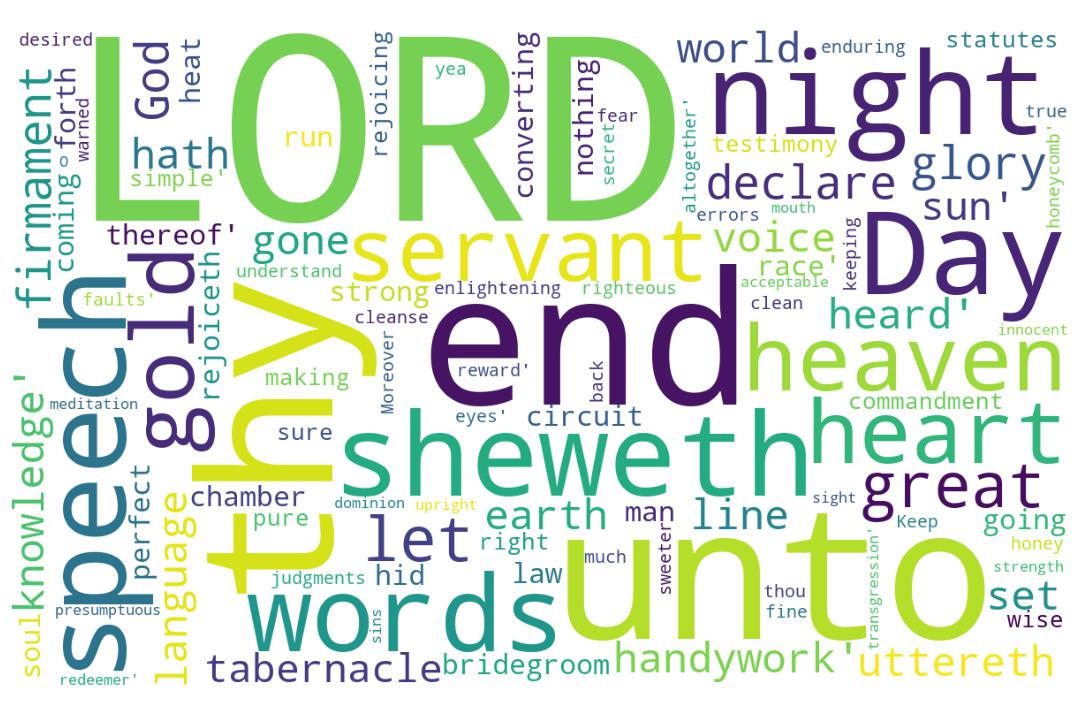
\includegraphics[width=\linewidth]{19OT-Psalms/Psalm19-WordCloud.jpg}
  \caption{Psalm 19 Word Cloud}
  \label{fig:Psalm 19 word Cloud}
\end{figure}

\marginpar{\scriptsize \centering \fcolorbox{bone}{lime}{\textbf{PROFITTING FROM REVELATION}}\\ Psalm 19:1-14) \begin{compactenum}[I.][8]
    \item \textbf{Revealing} \index[scripture]{Psalms!Psa 019:02}(Psa 19:2)
    \item \textbf{Redeeming} \index[scripture]{Psalms!Psa 019:07}(Psa 19:7)
    \item \textbf{Rejoicing} \index[scripture]{Psalms!Psa 019:08}(Psa 19:8)
    \item \textbf{Refreshing} \index[scripture]{Psalms!Psa 019:10}(Psa 19:10) (Sweet)
    \item \textbf{Rewarding} \index[scripture]{Psalms!Psa 019:11}(Psa 19:11)
    \item \textbf{Readying} \index[scripture]{Psalms!Psa 019:11}(Psa 19:11)
    \item \textbf{Refining} \index[scripture]{Psalms!Psa 019:12}(Psa 19:12)
\end{compactenum}}

\marginpar{\scriptsize \centering \fcolorbox{bone}{yellow}{\textbf{REVEALED TRUTH IS}}\\ Psalm 19:1-14) \begin{compactenum}[I.][8]
    \item \textbf{Communicated} \index[scripture]{Psalms!Psa 019:01}(Psa 19:1)
    \item \textbf{Continuous} \index[scripture]{Psalms!Psa 019:02}(Psa 19:2)
    \item \textbf{Indicative} \index[scripture]{Psalms!Psa 019:05}(Psa 19:5)
    \item \textbf{Climactic} \index[scripture]{Psalms!Psa 019:06}(Psa 19:6)
    \item \textbf{Converting} \index[scripture]{Psalms!Psa 019:07}(Psa 19:7)
    \item To be \textbf{Coveted} \index[scripture]{Psalms!Psa 019:10}(Psa 19:10)
    \item \textbf{Corrective} \index[scripture]{Psalms!Psa 019:11}(Psa 19:11)
\end{compactenum}}

\marginpar{\scriptsize \centering \fcolorbox{bone}{black}{\textbf{\textcolor[cmyk]{0,0,0,0}{WHAT HEAVENS DECLARE}}}\\ (Psalm 19:1-14)  
\begin{compactenum}[I.][8]
    \item \textbf{Reality}  -- hard to ignore!
    \item \textbf{Revelation} \index[scripture]{Psalms!Psa 019:01}(Psa 19:1)
    \item \textbf{A Return} \index[scripture]{Psalms!Psa 019:05}(Psa 19:5) -- bridegroom coming
    \item \textbf{A Requirement} \index[scripture]{Psalms!Psa 019:07-14}(Psa 19:7-14)
    \item \textbf{Rejoicing in God} \index[scripture]{Psalms!Psa 019:08}(Psa 19:8)
    \item \textbf{Righteousness} \index[scripture]{Psalms!Psa 019:09}(Psa 19:9)
    \item \textbf{A Reward for Obedience} \index[scripture]{Psalms!Psa 019:11}(Psa 19:11)
\end{compactenum}}

\marginpar{\scriptsize \centering \fcolorbox{bone}{blue}{\textbf{\textcolor[cmyk]{0,0,0,0}{REVELATION}}}\\ (Psalm 19:1-14)  
\begin{compactenum}[I.][8]
\item A Witness (Psa 19:3) 
\item Words (Psa 19:4)
\item Wisdom (Psa 19:7) 
\item A Warning (Psa 19:11)
\item Wonder
\end{compactenum}}

\footnote{\textcolor[cmyk]{0.99998,1,0,0}{\hyperlink{TOC}{Return to end of Table of Contents.}}}\footnote{\href{https://www.audioverse.org/english/audiobibles/books/ENGKJV/O/Ps/1}{\textcolor[cmyk]{0.99998,1,0,0}{Psalms Audio}}}\textcolor[cmyk]{0.99998,1,0,0}{To the chief Musician, A Psalm of David.}\\
\\
\textcolor[cmyk]{0.99998,1,0,0}{The heavens \fcolorbox{bone}{yellow}{declare} the glory of God; and the firmament sheweth his handywork.}\footnote{\textbf{Genesis 1:6-7} - And God said, Let there be a firmament in the midst of the waters, and let it divide the waters from the waters. [7] And God made the firmament, and divided the waters which were under the firmament from the waters which were above the firmament: and it was so. 8 And God called the firmament Heaven. And the evening and the morning were the second day.}
[2] \textcolor[cmyk]{0.99998,1,0,0}{\fcolorbox{bone}{yellow}{Day unto day} uttereth speech, and night unto night \fcolorbox{bone}{lime}{sheweth} \fcolorbox{bone}{lime}{knowledge}.}
[3] \textcolor[cmyk]{0.99998,1,0,0}{\emph{There} \emph{is} no speech nor language, \emph{where} their voice is not heard.}
[4] \textcolor[cmyk]{0.99998,1,0,0}{Their line is gone out through all the earth, and their words to the end of the world. In them hath he set a tabernacle for the sun,}
[5] \textcolor[cmyk]{0.99998,1,0,0}{Which \emph{is} \fcolorbox{bone}{yellow}{as a bridegroom} coming out of his chamber, \emph{and} rejoiceth as a strong man to run a race.}\footnote{\textbf{Joel 2:16} -  Gather the people, sanctify the congregation, assemble the elders, gather the children, and those that suck the breasts: let the bridegroom go forth of his chamber, and the bride out of her closet.}
[6] \textcolor[cmyk]{0.99998,1,0,0}{His going forth \emph{is} from the end of the heaven, and his circuit \fcolorbox{bone}{yellow}{unto the ends of it}: and there is nothing hid from the heat thereof.}
[7] \textcolor[cmyk]{0.99998,1,0,0}{The law of the LORD \emph{is} perfect, \fcolorbox{bone}{lime}{converting} the soul: the testimony of the LORD \emph{is} sure, making wise the simple.}
[8] \textcolor[cmyk]{0.99998,1,0,0}{The statutes of the LORD \emph{are} right, \fcolorbox{bone}{lime}{rejoicing} the heart: the commandment of the LORD \emph{is} pure, enlightening the eyes.}\footnote{\textbf{Ephesian 1:18} - The eyes of your understanding being enlightened; that ye may know what is the hope of his calling, and what the riches of the glory of his inheritance in the saints,}
[9] \textcolor[cmyk]{0.99998,1,0,0}{The fear of the LORD \emph{is} clean, enduring for ever: the judgments of the LORD \emph{are} true \emph{and} righteous altogether.}
[10] \textcolor[cmyk]{0.99998,1,0,0}{More \fcolorbox{bone}{yellow}{to be desired} \emph{are} \emph{they} than gold, yea, than much fine gold: \fcolorbox{bone}{lime}{sweeter} also than honey and the honeycomb.}
[11] \textcolor[cmyk]{0.99998,1,0,0}{Moreover by them is thy servant \fcolorbox{bone}{lime}{warned}: \emph{and} in keeping of them \emph{there} \emph{is} great \fcolorbox{bone}{lime}{reward}.}
[12] \textcolor[cmyk]{0.99998,1,0,0}{Who can understand \emph{his} errors? \fcolorbox{bone}{lime}{cleanse} thou me from secret \emph{faults}.}\footnote{\textbf{Jeremiah 17:9} - The heart is deceitful above all things, and desperately wicked: who can know it?}
[13] \textcolor[cmyk]{0.99998,1,0,0}{Keep back thy servant also from presumptuous \emph{sins}; let them not have dominion over me: then shall I be upright, and I shall be innocent from the great \fcolorbox{bone}{MYGOLD}{transgression}.}\marginpar{\scriptsize \textcolor[rgb]{0.00,0.545,0.269}{$\rightarrow$Described(1) law of the Lord (vs 7) (2) testimony of the Lord)  (vs 7) , (3) statutes of the Lord  (vs 8) , (4) commandment of the Lord  (vs 8) , (5) fear of the Lord  (vs 9) , and (6) judgments of the Lord (vs 9).}}
[14] \textcolor[cmyk]{0.99998,1,0,0}{Let the words of my mouth, and the meditation of my heart, be acceptable in thy sight, O LORD, my strength, and my redeemer.}
%\marginpar{\textcolor[rgb]{0.13, 0.55, 0.13}{\tiny What Creation Provides: \begin{compactenum}[I.][7]
%\end{compactenum} } } 

